\documentclass{beamer}
\usepackage{ctex, hyperref}
\usepackage[T1]{fontenc}

% other packages
\usepackage{latexsym,amsmath,xcolor,multicol,booktabs,calligra}
\usepackage{graphicx,pstricks,listings,stackengine}

\author{userElaina}
\title{BlackVIP
}
\subtitle{Black-Box Visual Prompting for Robust Transfer Learning}
\institute{JLU-SAI}
\date{2024.04.12}
\usepackage{JilinUniv}

% defs
\def\cmd#1{\texttt{\color{red}\footnotesize $\backslash$#1}}
\def\env#1{\texttt{\color{blue}\footnotesize #1}}
\definecolor{deepblue}{rgb}{0,0,0.5}
\definecolor{deepred}{rgb}{0.6,0,0}
\definecolor{deepgreen}{rgb}{0,0.5,0}
\definecolor{halfgray}{gray}{0.55}

\lstset{
    basicstyle=\ttfamily\small,
    keywordstyle=\bfseries\color{deepblue},
    emphstyle=\ttfamily\color{deepred},    % Custom highlighting style
    stringstyle=\color{deepgreen},
    numbers=left,
    numberstyle=\small\color{halfgray},
    rulesepcolor=\color{red!20!green!20!blue!20},
    frame=shadowbox,
}


\begin{document}

\kaishu
\begin{frame}
    \titlepage
    \begin{figure}[htpb]
        \begin{center}
            
\includegraphics[width=0.15\linewidth]{pic/Jilin_University_Logo.eps}
        \end{center}
    \end{figure}
\end{frame}

\begin{frame}
\tableofcontents[sectionstyle=show,subsectionstyle=show/shaded/hide,subsubsectionstyle=show/shaded/hide]
\end{frame}

\section{Introduction}

\begin{frame}{Visual Prompting}
    \begin{itemize}[<+-| alert@+>]
        \item 1234+2345*3333+4567?
        \item step by step. 1234+2345*3333+4567?
        \item alfa bravo charlie david 1234+2345*3333+4567?
        \item Visual Prompting
    \end{itemize}
\end{frame}

\begin{frame}{Black-Box PTM}
    \begin{figure}[l]
        \centering
        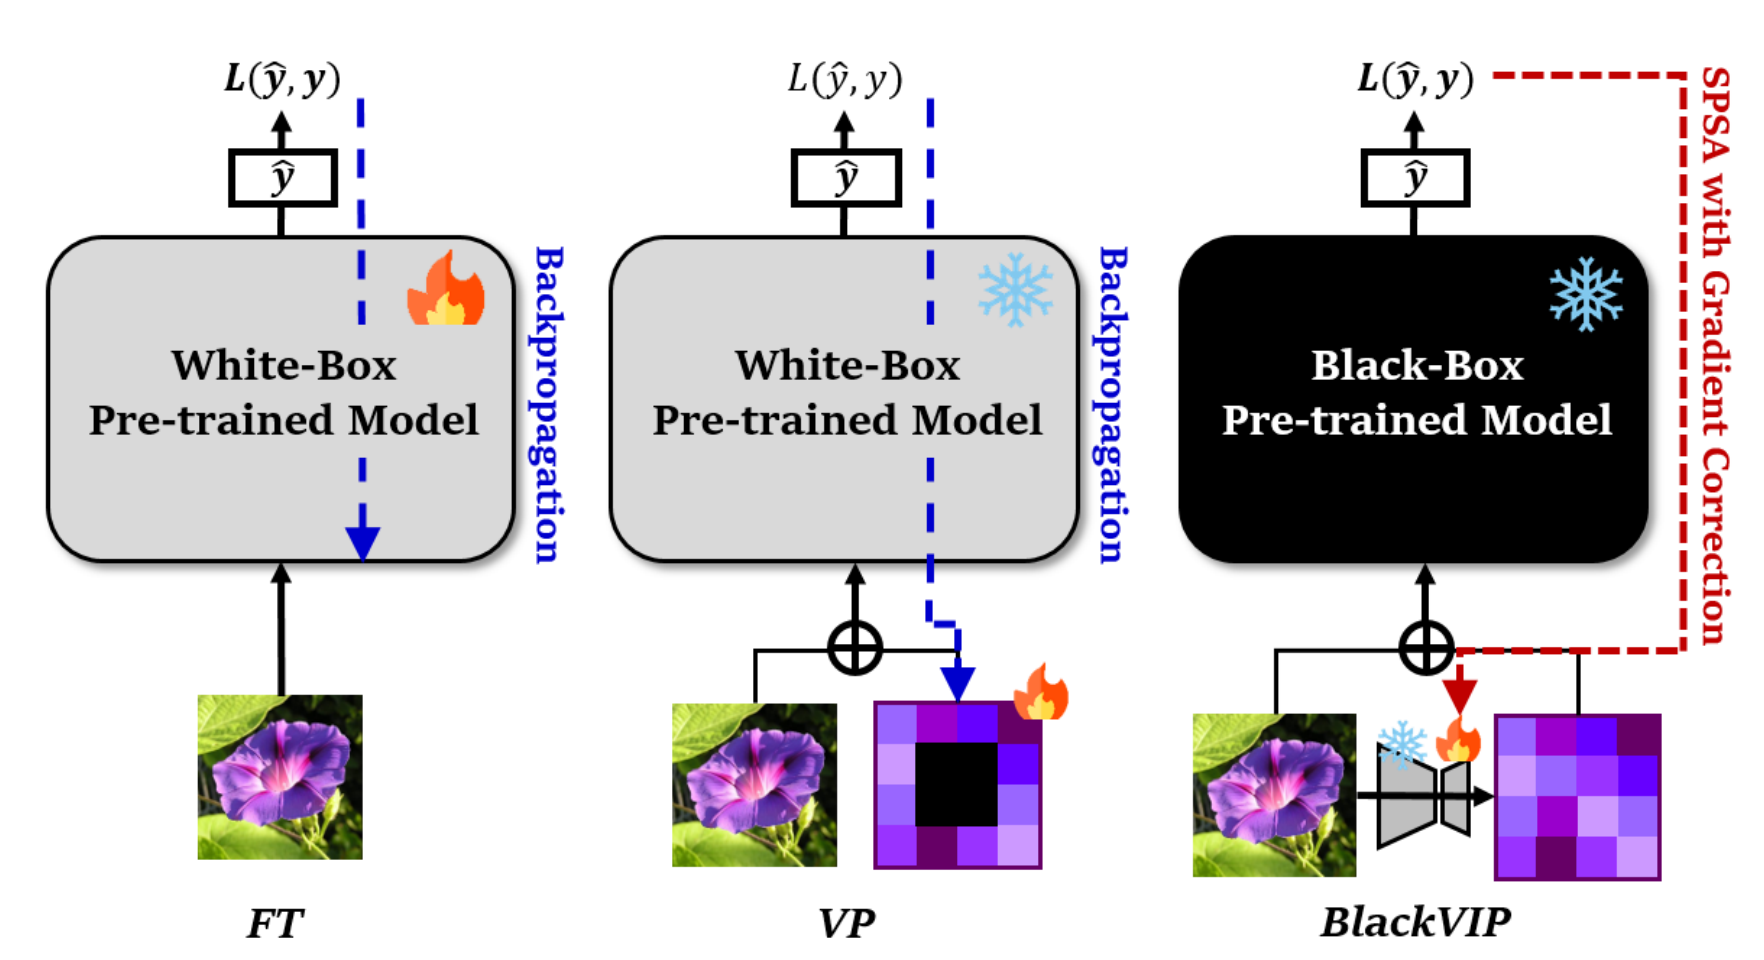
\includegraphics[width=\textwidth]{pic/1.png}
        % \caption{PTM}
    \end{figure}
\end{frame}

\section{Methodology}

\begin{frame}{BlackVIP}
    \begin{figure}[l]
        \centering
        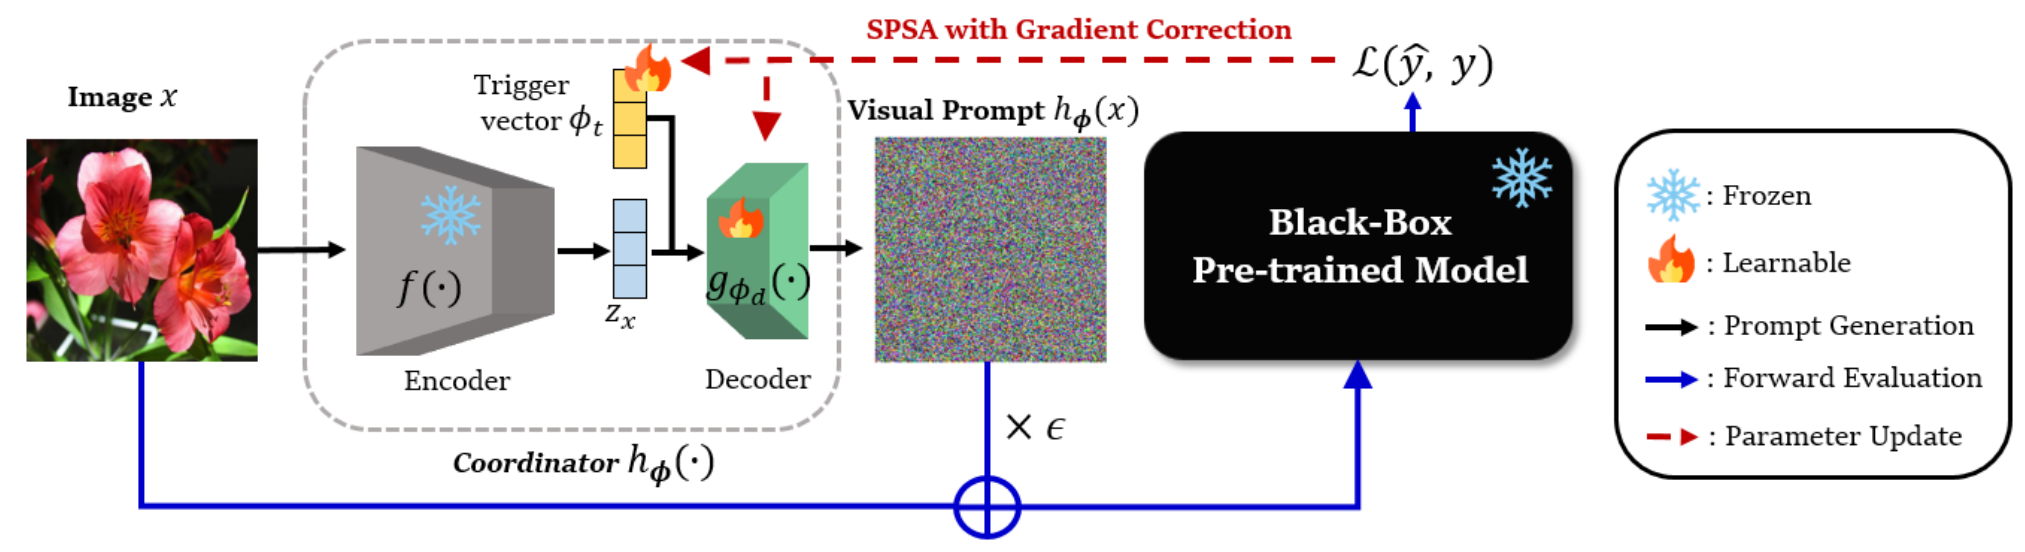
\includegraphics[width=\textwidth]{pic/2.png}
        % \caption{BlackVIP}
    \end{figure}
\end{frame}

\begin{frame}{Coordinator}
    \begin{itemize}
        \item Encoder: frozen, pre-trained on ImageNet by SSL.
        \par \begin{equation*}
            \begin{aligned}
                Z_x=f(x)
            \end{aligned}
        \end{equation*}
        \item Decoder: prompt generation network.
        \par \begin{equation*}
            \begin{aligned}
                h_{\varPhi_i}(x)=g_{\varPhi_{d,i}} (Z_x,\varPhi_{t,i})
            \end{aligned}
        \end{equation*}
        \item CLIP: It can be instructed in natural language to predict the most relevant text snippet, given an image, without directly optimizing for the task, similarly to the zero-shot capabilities of GPT-2 and 3.
        \par \begin{equation*}
            \begin{aligned}
                \hat{x}=\rm{clip}(x+\varepsilon h_{\varPhi_i}(x))
            \end{aligned}
        \end{equation*}
    \end{itemize}
\end{frame}

\begin{frame}{SPSA}
    \begin{figure}[l]
        \centering
        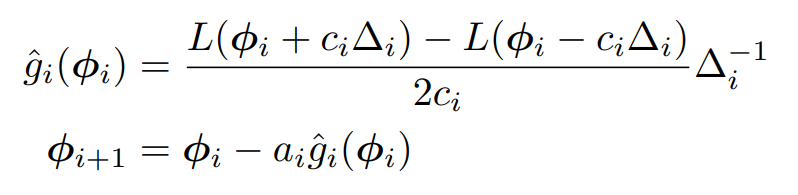
\includegraphics[width=\textwidth]{pic/3.png}
        % \caption{SPSA}
    \end{figure}
\end{frame}

\begin{frame}{SPSA-GC}
    \begin{figure}[l]
        \centering
        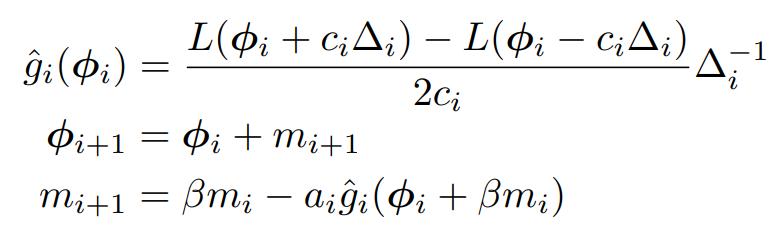
\includegraphics[width=\textwidth]{pic/4.png}
        % \caption{SPSA-GC}
    \end{figure}
\end{frame}

\begin{frame}{BlackVIP}
    \begin{figure}[l]
        \centering
        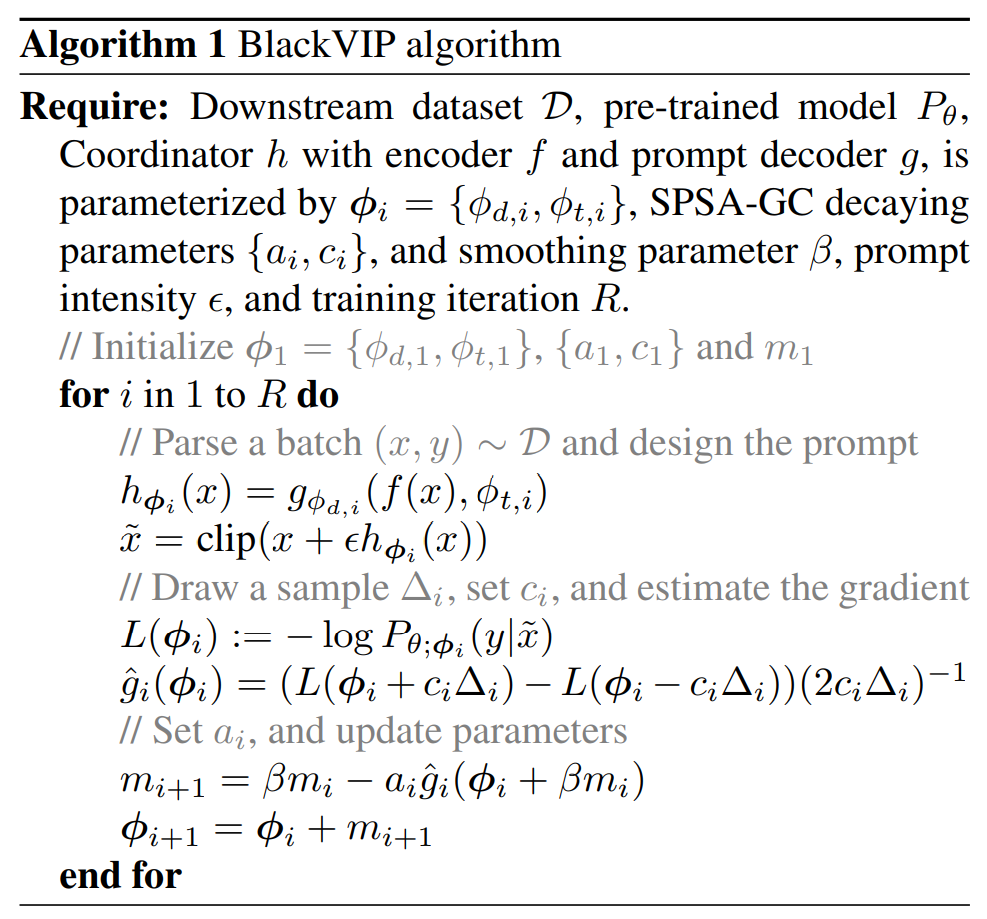
\includegraphics[height=.8\textheight]{pic/5.png}
        % \caption{BlackVIP}
    \end{figure}
\end{frame}

\end{document}
